\section{Short and long response functions}\label{sec:short_long}

Regarding Equation \ref{eq:return_general}, we use a time lag $\tau$ in the
returns to see the gains or loses in a future time. However, the strength of
the return in the time lag should not be equal along its length. Then, we
divide the full range time lag $\tau$ in an immediate time lag and in a late
time lag as show in Fig. \ref{fig:tau_short_long}, where

\begin{equation}\label{eq:tau_short_long}
    \tau = \tau' + \left( \tau - \tau' \right)
\end{equation}

for $\tau' < \tau$. This distinguish the returns depending in the time lag as
the short (immediate) return $\tau'$ with the long return $\tau - \tau'$.

\begin{figure}[htbp]
    \centering
    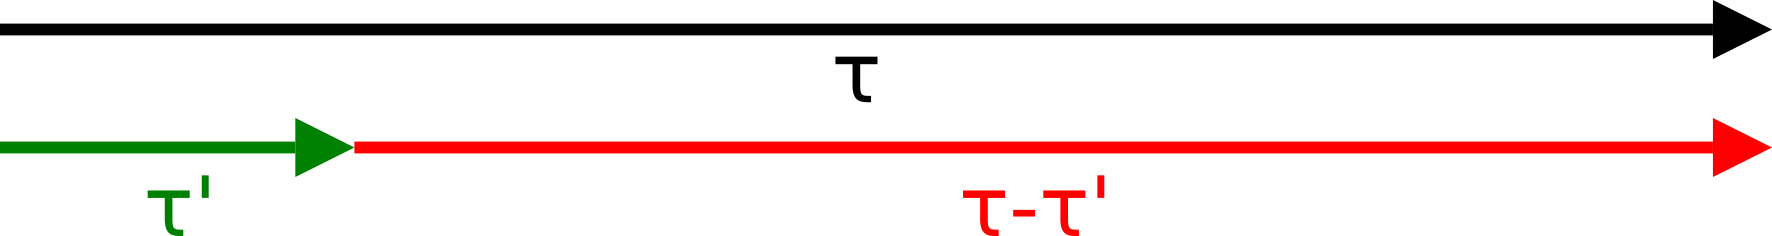
\includegraphics[width=\columnwidth]{figures/05_tau_short_long.png}
    \caption{$\tau$ value divided in short and long time lag.}
    \label{fig:tau_short_long}
\end{figure}

To use the short and long time lag, we rewrite the returns in physical time
scale as

\begin{align}\label{eq:short_long_return}
    r^{sl,p}_{i}\left(t,\tau\right)&=\ln\left(\frac{m_{i}\left(t+\tau\right)}
    {m_{i} \left(t\right)}\right) \nonumber \\
    &=\ln\left(\frac{m_{i}\left(t+\tau\right)}{m_{i}\left(t+\tau'\right)}
    \cdot\frac{m_{i} \left(t+\tau'\right)}{m_{i}\left(t\right)}\right)
    \nonumber \\
    &=\ln\left(\frac{m_{i}\left(t+\tau\right)}{m_{i}\left(t+\tau'\right)}
    \right)+ \ln\left(\frac{m_{i}\left(t+\tau'\right)}{m_{i}\left(t\right)}
    \right)\nonumber \\
    &\approx\frac{m_{i}\left(t+\tau\right)-m_{i}\left(t+\tau'\right)}
    {m_{i}\left(t+\tau'\right)} +\frac{m_{i}\left(t+\tau'\right)-m_{i}
    \left(t\right)}{m_{i}\left(t\right)}
\end{align}

where $sl$ refers to short-long and the second term of the right part is
constant with respect to $\tau$. Replacing Equation \ref{eq:short_long_return}
in the response function (Eq. \ref{eq:response_functions_time_scale_general})
we have

\begin{align}\label{eq:short_long_response}
    R^{sl,p}_{ij}\left(\tau\right)&=\left\langle
    r^{sl,p}_{i}\left(t - 1, \tau\right)
    \cdot\varepsilon^{p}_{j}\left(t\right)\right\rangle _{p} \nonumber \\
    &\approx\left\langle \frac{m_{i}\left(t - 1 +\tau\right)-m_{i}
    \left(t - 1 +\tau'\right)} {m_{i}\left(t - 1 +\tau'\right)}
    \cdot\varepsilon_{j} \left(t\right)\right\rangle _{p} \nonumber \\
    & +\left\langle \frac{m_{i} \left(t - 1 +\tau'\right)-m_{i}
    \left(t - 1\right)}{m_{i}\left(t - 1\right)}
    \cdot\varepsilon_{j}\left(t\right)\right\rangle _{p}
\end{align}

Where the first term in the right side of Equation \ref{eq:short_long_response}
is the long response and the right term is the short response. Again, the right
term of Equation \ref{eq:short_long_response} is independent of $\tau$.

\begin{figure*}[htbp]
    \centering
    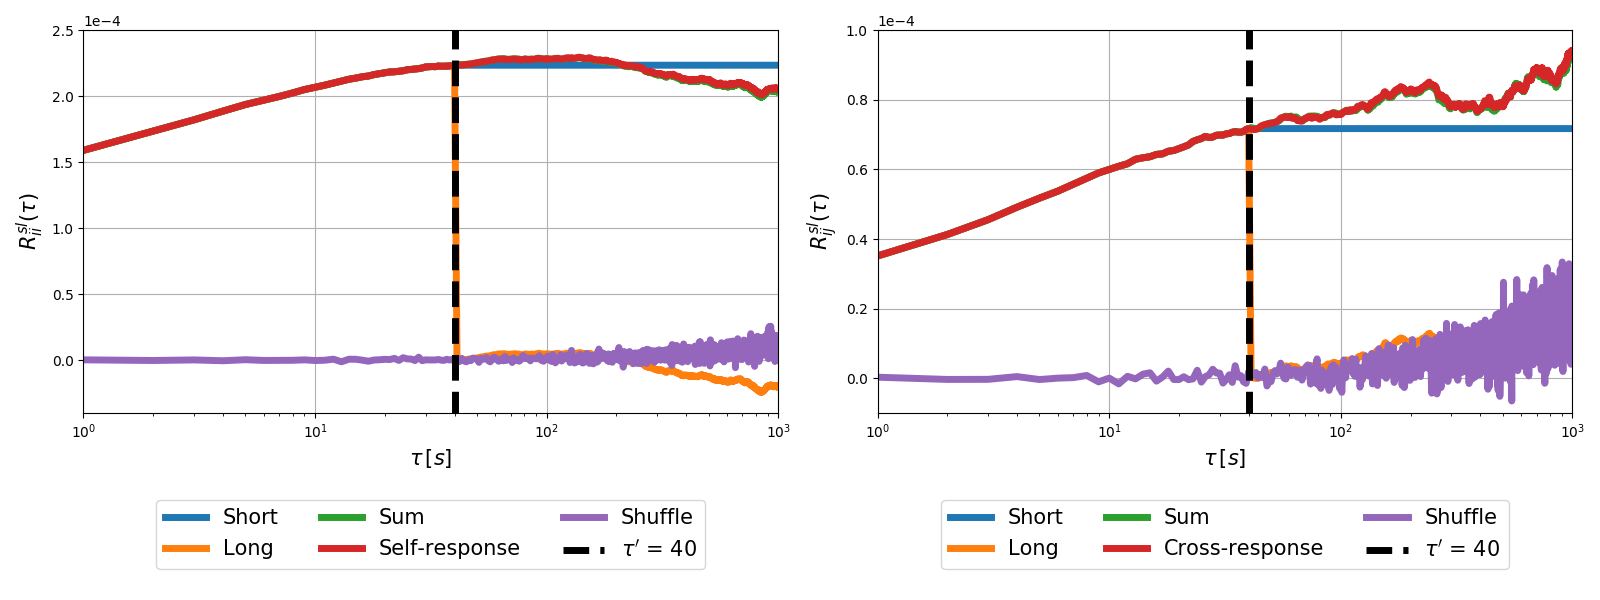
\includegraphics[width=\textwidth]
    {figures/05_short_long_GOOG_MA.png}
    \caption{Self- and cross-response functions
             $R^{sl,p}_{ij}\left(\tau\right)$ excluding
             $\varepsilon^{p}_{j}\left(t\right) = 0$ in 2008 versus time lag
             $\tau$ on a logarithmic scale using a $\tau'=40$ in physical time
             scale. Self-response functions (left) of Alphabet Inc. stock and
             cross-response functions (right) of Alphabet Inc.-Mastercard Inc.
             stocks.}
    \label{fig:short_long_responses}
\end{figure*}

The results in Fig. \ref{fig:short_long_responses} show the short response, the
long response, the addition of the short response and long response (Sum), the
original response, a random response and the value of $\tau'$.

The main signal of the response function come from the short response.
Depending on the stock and the value of $\tau'$ the long response can increase
or decrease the short response signal, but in general the long response does
not give a significant contribution to the complete response.

Before $\tau'$, the short response and long response are the same, as the self
and cross-response definition do not define values smaller than $\tau '$, so it
is computed as the original response. In the figure, the curves of the short
and long response are under the curve of the original response. After $\tau'$,
the short response is a strong constant signal. On the other hand, the long
response immediately fades, showing the small contribution to the final
response. To compare the significance of the long response, We added a random
response made with the trade signs used to compute the response but with a
shuffle order. The long response and the random response are comparable, and
show how the long response is not that representative in the final response.
If we add the short and long response, we obtain the original response. In Fig.
\ref{fig:short_long_responses}, the original response (red line) has the same
shape to the addition of the short and long response (green line).

For the response functions that show the increase-decrease behavior in between
the time lag $\tau = 10^{3}$, the peak is usually between $\tau = 10^{1}$ and
$\tau = 10^{2}$. In these cases the long response are always negative after the
$\tau'$ value and is comparable in magnitude with the random signal.

On the other hand, the response functions that requires a bigger time lag to
show the increase-decrease behavior, have non negative long responses, but
still they are comparable in magnitude with the random signal.